\documentclass[10pt, reqno]{article}
\usepackage{amsmath}
\usepackage{amsfonts}
\usepackage{amssymb}
\usepackage{amsthm}
%american mathematical society - AMS 

\usepackage{hyperref}
\usepackage{float}
\usepackage{enumerate}
\usepackage{graphicx}
\usepackage{wrapfig}
\usepackage{subfig}

\oddsidemargin = 0in
\textwidth=6.5in

\numberwithin{equation}{section} 

\numberwithin{figure}{section}

\title{The Trapezoidal rule}
\author{Johnny Minor}
\date{\today}

\begin{document}

\maketitle

\section{Introduction}
Beyond the pages of introductory calculus textbooks mathematicians, engineers, and physicists will frequently encounter functions that are integrable, but do not have antiderivatives. As we know quite well the integral of a function can be thought of as the area underneath that specific curve. This geometric interpretation of the integral can be leveraged when dealing with functions that are not well behaved. 
In order to use this geometric interpretation we employ trapezoids, and a computer program to solve for the integral. 

\section{Trapezoids}
\label{sec:trapz}

Trapezoids seem like a reasonable shape to use to find the sum of an unknown area. This is because the characteristics of trapezoids lend well to conforming to many different shapes. Often times functions that are not well behaved end up being very strange shapes. In comparison to a well behaved periodic function such as $y = \sin(x) $ or $y = \cos(x)$. Figure \ref{fig:trapz} is an illustration of how many different shapes and sizes that a trapezoid can take on depending on the length of its sides and also the angle in the corners. 


\begin{figure}[H] % 'h' means put it here and 'ht' means that put it at top the and here. 'ht!' put it here now! 
\centering
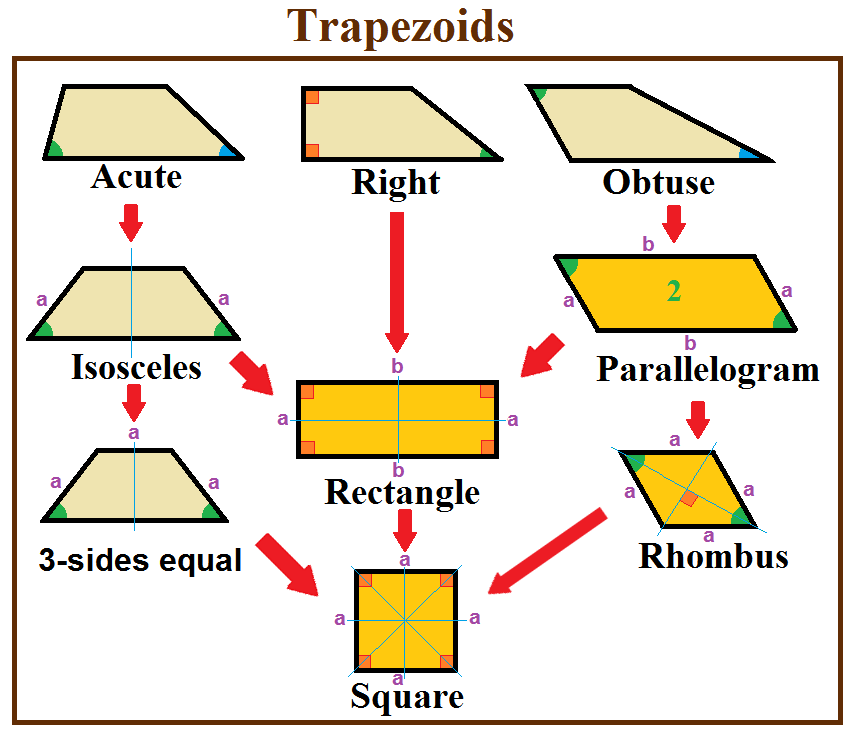
\includegraphics[width=0.4\textwidth]{Trapezoid_special_cases.png}
\caption{Special cases of trapezoids\cite{ref:trapz}}
\label{fig:trapz}
\end{figure}

\noindent Figure \ref{fig:trapz} should be taken as clear motivation for why we use trapezoids instead of triangles, or octahedrons. 
Furthermore, we choose trapezoids because when we have a function $f(x)$ we can easily calculate two adjacent points. From these two points we can then form a trapezoid. This is essentially what the two point trapezoidal rule is.  

\section{The Trapezoid Rule}

To begin with the trapezoid rule we first define the area of integration to be the closed interval $[a,b]$. We then divide this interval into $h$ sections. 
\begin{equation}
\label{eq:meshspacing}
h = \frac{b-a}{n}
\end{equation}

\noindent Where $n$ is the number of intervals, $b$ is the end of interval and $a$ is the beginning of the interval, and $h$ is how large each interval will be. $h$ is often referred to as the mesh spacing. We have now determined how large each section in the interval should be in order to be equal. This means we need  $n + 1$ points. We will evaluate the function we are trying to integrate at these points.

A natural question arises about why we need $n+1$ points. This is a common snag in many people's intuitive understanding of dividing an interval into equal sections, and is often referred to as the "Fencepost error" in Applied Mathematics and Computer Science. For example: 

\medskip

\noindent \textit{If you want to build a straight fence 30 meters long with posts spaced 3 meters apart, how many posts do you need?}     

\medskip

\noindent Well, the intuitive answer for most people is to think: $30/3 = 10$ so we must need 10 posts. Unfortunately that is not correct, and we really need 11 posts! If you don't believe me you can look at this diagram

\begin{figure}[ht!] % 'h' means put it here and 'ht' means that put it at top the and here. 'ht!' put it here now! 
\centering
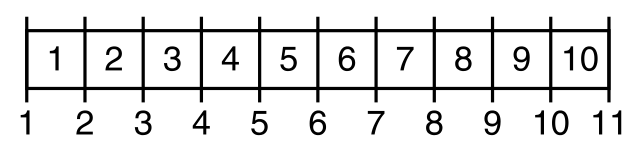
\includegraphics[width=0.4\textwidth]{Fencepost.png}
\caption{An illustration on the fence post problem \cite{ref:fencepost}}
\label{fig:fencepost}
\end{figure}

\noindent This shows without question that we will indeed $n+1$ points in order to create our trapezoids with spacing of $h$. 

Now that we have split out interval into intervals we need to form our trapezoids. First, our points which we will evaluate our function at will be defined as 

$$ 
x_0 = a, x_1 = a + \Delta x, x_2 = a + 2\Delta x, \dots x_n = a + n\Delta x = b. 
$$

From these $x$ values we need to calculate the corresponding output of our function of interest. This will look like 
$$
y_0 = f(x_0), y_1 = f(x_1), y_2 = f(x_2), \dots, y_n = f(x_n) 
$$ 

Now that we have the $x$ values and the $y$ values we can then form $n$ trapezoids throughout or closed interval. To find the area of a trapezoid by breaking our trapezoid into a square of length $y_0$ and then a right triangle with height $y_1 - y_0$. This expression will be 

\begin{equation}
\label{eq:area}
A = y_0 h + \frac{1}{2}(y_1 - y_0)h.
\end{equation}

The first term in the sum is the area of the square, and the second term is the area of the left over triangle. In equation \ref{eq:area} $A$ is the area of the trapezoid $y_0$ is $f(x_0)$ analogously $y_1$ is $f(x_1)$, and $h$ is the mesh spacing from equation \ref{eq:meshspacing}(or change in $x$ between adjacent trapezoids). 
If we apply this area to our $n$ trapezoids we end up with the expression 

\begin{equation}
\int_{a}^{b} f(x)dx \approx \frac{(y_0 + y_1)h}{2} + \frac{(y_1 + y_2)h}{2} + \frac{(y_2 + y_3)h}{2} + \cdots + \frac{(y_n + y_n)h}{2}
\end{equation}

\noindent With some work this will simplify to the trapezoidal rule formula. 

\begin{equation}
\int_{a}^{b} f(x) \approx \frac{h}{2}(y_0 + 2y_1 + 2y_2 + \cdots + 2y_{n-1} + y_n)
\end{equation}
 
\theoremstyle{definition}
\newtheorem{exmp}{Example}[section]

\begin{exmp}
Consider the function $f(x) = \cos(x)$ on the closed interval $[0,\pi/2]$. If we choose $n$ equal to 3 then the function with the trapezoids will look like this 

\begin{figure}[H] % 'h' means put it here and 'ht' means that put it at top the and here. 'ht!' put it here now! 
\centering
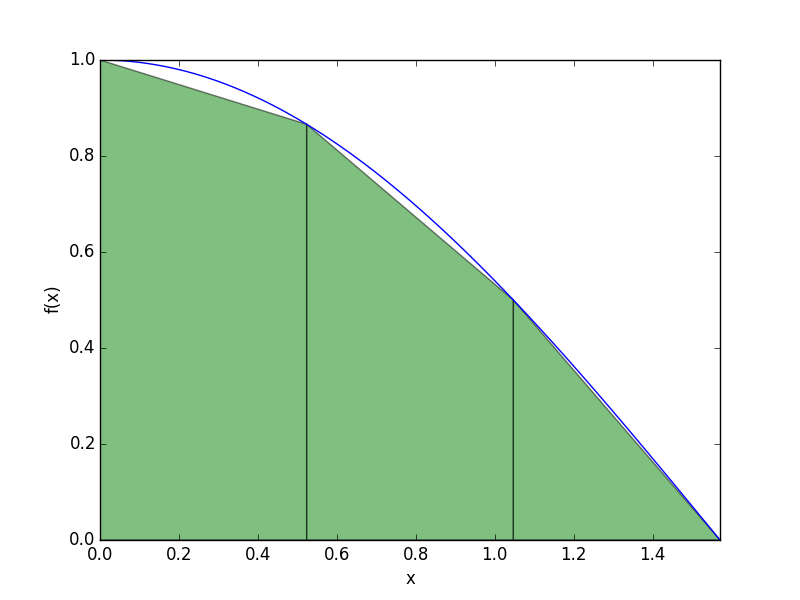
\includegraphics[width=0.4\textwidth]{HW6-plot.png}
\caption{Trapezoidal Rule on 3 Subintervals}
\label{fig:cosine_example}
\end{figure}

It should be noted that when $n$ is chosen to be relatively small that the trapezoidal rule will underestimate a function that is concave down on the interval and alternatively will overestimate a function that is concave up. This can be seen by inspection of the unaccounted white space seen in figure \ref{fig:cosine_example}. 
The error equation for the Trapezoidal Rule is\cite{ref:Atkinson}  

\begin{equation}
\label{eq:error}
E_{n}^{T}(f) \equiv \int_{a}^{b} f(x) dx - T_n(f) = - \frac{h^2 (b-a)}{12} f''(c_n).
\end{equation}

\noindent Equation\ref{eq:error} shows that the error decreases approximately proportional to to $h^2$. Therefore, if $n$ is doubled and therefor halving $h$. The resulting error would be approximately $2^2$ or 4.\cite{ref:Atkinson}  

\begin{table}[H]
\begin{center}
\caption{Trapezoidal Rule for $f(x)$}
\begin{tabular}{|c|l c|}
\hline
\boldmath$2h/\pi$ & \multicolumn{1}{|c}{\textbf{Integral}} & \multicolumn{1}{c|}{\textbf{Error}} \\ \hline 
%\rule{0pt}{3ex} this would add more vertical space, but I don't really like it... 
$10^{-1}$ & 0.99794299 & $2.057 \times 10^{-3}$ \\ 
$10^{-2}$ & 0.99997944 & $2.056 \times 10^{-5}$ \\ 
$10^{-3}$ & 0.9999979 & $2.056 \times 10^{-7}$ \\ 
$10^{-4}$ & $\sim 1$ & $2.056 \times 10^{-9} $\\
$10^{-5}$ & $\sim 1$ & $2.057 \times 10^{-11}$ \\  
\hline
\end{tabular}
\end{center}
\end{table}


\noindent As we increase $n$ it can be seen that precision increases quickly, and with large enough $n$(or small $h$) converge to the analytic solution of 1. Naysayers might protest noting that we could have integrated $f(x) = \cos(x)$ easily and found the analytic solution with considerably less work. However, we have proven that the trapezoidal rule is a very accurate method for integrating periodic functions without anti derivatives. 

\end{exmp}


\section{Conclusion}

We have motivated the use of trapezoids rather than other geometric objects. They are able to change shape to match many different features found in functions. We then developed the general expression for the Trapezoid Rule for a general function $f(x)$ on a closed interval $[a,b]$. We then illustrated the usage of the Trapezoidal Rule on the function $f(x) = \cos(x)$ on $[0,\pi/2]$, and showed that using the Trapezoidal Rule the solution can be found to be the same as the analytic solution. Thus proving that the Trapezoidal Rule is indeed an accurate and effective method for calculating the integral of functions without anti derivatives. 



\begin{thebibliography}{XX}

\bibitem{ref:trapz} %when we refer to it by name we use this name. 
Tomruen(\url{https://commons.wikimedia.org/wiki/File:Trapezoid_special_cases.png})[Public Domain], via Wikimedia Commons

\bibitem{ref:fencepost} %when we refer to it by name we use this name. 
Acdx (\url{https://commons.wikimedia.org/wiki/File:Fencepost_error.svg})[Public Domain], via Wikimedia Commons

\bibitem{ref:Cazelais}
Gilles Cazelais, \textbf{The Trapezoid Rule}, Camosun College, Victoria, British Columbia, \today. 

\bibitem{ref:Atkinson}
Kendall E Atkinson, \textbf{Trapezoidal Method Error Formula}, University of Iowa, Iowa City, Iowa, \today.
\end{thebibliography} 




\end{document}